\documentclass[11pt]{article}
\usepackage[margin=1in]{geometry}
\usepackage{amsmath, amssymb, mathtools}
\usepackage{enumitem}
\usepackage{graphicx}   % <-- needed for \includegraphics
\usepackage{float}      % <-- for [H] placement
\usepackage{hyperref}   % <-- load last

\title{\textbf{ECE 506: Homework \#1: Basic Optimization}}
\date{}

\begin{document}
	
	\maketitle
	
	\noindent
	To get help with the homework, please join the Saturday morning discussion sessions starting at 9am at
	\url{https://unm.zoom.us/j/99977790315}.\\
	
	\textbf{Problem \#1. An Introduction to Linear Programming}
	
	This problem is focused on manipulating the basic Linear Programming equation:
	\begin{equation}
		\min_{x}\; c^{\top}x
		\quad \text{subject to } Ax = b \text{ and } x \ge 0.
		\label{eq:lp}
	\end{equation}
	(Here, $x \ge 0$ is understood componentwise.)
	
	\begin{enumerate}[label=\textbf{1(\alph*)}]
		
		\item \textbf{Problem statement.}
		We begin with the simplest possible example! Consider the 1D problem:
		\begin{equation}
			\min_{x}\; c \cdot x
			\quad \text{subject to } a x = b \text{ and } x \ge 0.
			\label{eq:1d}
		\end{equation}
		From this case, answer the following:
		\begin{enumerate}[label=\roman*)]
			\item Give an example where there is no solution.
			\item Give an example with a simple solution.
			\item For your solution, did you minimize anything? Explain.
		\end{enumerate}
		
		\textbf{Solution.}
		With the constraints \(ax=b\) and \(x\ge 0\), if \(a\neq 0\) then the only candidate is
		\(x^\star=\tfrac{b}{a}\).
		\begin{enumerate}[label=\roman*)]
			\item If \(b/a<0\), the nonnegativity constraint is violated, so the problem is infeasible; e.g.,
			\(a=1,\ b=-1 \Rightarrow x^\star=-1\) (infeasible).
			(Also infeasible when \(a=0,\ b\neq 0\) since \(0=b\) cannot hold.)
			\item Example with a simple solution: Take \(a=2,\ b=0\). Then \(x^\star=\tfrac{b}{a}=0\), which satisfies \(x\ge 0\), and the objective value is \(c\,x^\star=0\).
			\item Did we minimize anything? No. When \(a\neq 0\), the equality constraint pins down a single feasible point \(x^\star\);
			if it is feasible, it is automatically optimal—there is no tradeoff to optimize over.
		\end{enumerate}
		
		\item \textbf{Problem statement.}
		More generally, consider $Ax = b$ for many dimensions. Suppose that $A$ is invertible. In this case, show that there is no minimization! To show this, compute the solution without minimizing $c^{\top}x$.
		
		\textbf{Solution.}
		If $A$ is invertible, the constraint $Ax=b$ has the unique solution $x^\star=A^{-1}b$. If $x^\star\ge 0$ (componentwise), it is the only feasible—and thus optimal—point with value $c^\top x^\star$; otherwise the problem is infeasible. No minimization needed.
		
		\item \textbf{Problem statement.}
		The only case that is interesting is when we have many solutions to $Ax = b$. We then get to pick the one that minimizes $c^{\top}x$. This can only happen when the number of equations is smaller than the number of unknowns. Here is an example:
		\[
		\begin{bmatrix} 1 & 2 \end{bmatrix}
		\begin{bmatrix} x_1 \\ x_2 \end{bmatrix} = 2.
		\]
		Note that we have one equation in two unknowns. We have more unknowns than we have equations! It may be possible to set up a proper optimization problem.
		
		To have a proper solution, we must also satisfy $x_1, x_2 \ge 0$. These are called \emph{feasible solutions}. They satisfy the constraints, and the optimal solution needs to satisfy them.
		
		\textbf{Task:} Plot all possible solutions of $Ax = b$ satisfying $x_1, x_2 \ge 0$ for this case.
		
		\textbf{Solution.}
		The feasible set is
		\[
		\{(x_1,x_2)\in\mathbb{R}^2_{\ge 0} \mid x_1 + 2x_2 = 2\},
		\]
		which is the line segment in the first quadrant between the intercepts $(2,0)$ and $(0,1)$. Any feasible point can be written as
		\[
		(x_1,x_2) = (2-2t,\ t), \quad t\in[0,1].
		\]
		A plot of this segment (restricted to $x_1,x_2\ge 0$) depicts the feasible region.
		
		\begin{figure}[H]
			\centering
			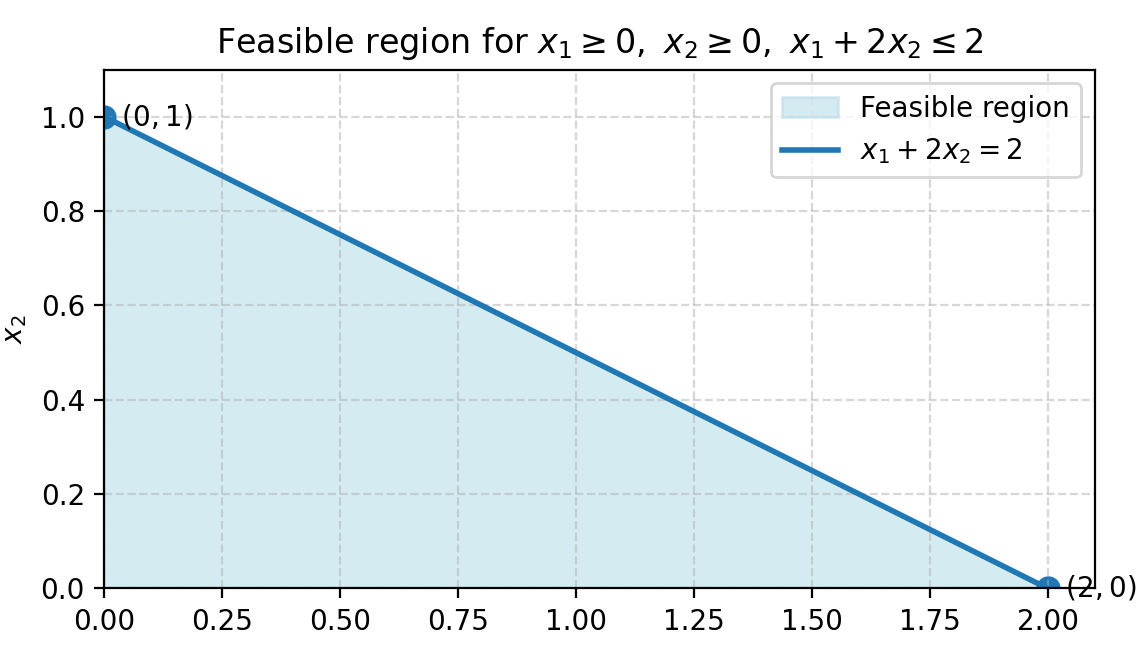
\includegraphics[width=\textwidth]{1c.png}
			\caption{Feasible region for $x_1 + 2x_2 = 2$ with $x_1, x_2 \geq 0$.}
		\end{figure}
		
		\item \textbf{Problem statement.}
		For the case when $Ax = b$ described in 1(c), solve the proper optimization problem. For this case, solve:
		\begin{equation}
			\min_{x}\; [\,1\;\;1\,]\,x
			\quad \text{subject to } Ax = b \text{ and } x \ge 0.
			\label{eq:obj11}
		\end{equation}
		Is the solution at the endpoints? Explain.
		
		\textbf{Solution.}
		The feasible set is $\{(x_1,x_2): x_1+2x_2=2,\; x_1,x_2\ge 0\}$, i.e., the segment between $(2,0)$ and $(0,1)$.
		Along this line, substitute $x_1=2-2x_2$ into the objective $x_1+x_2$ to get
		\[
		x_1 + x_2 = (2 - 2x_2) + x_2 = 2 - x_2.
		\]
		Over $x_2 \in [0,1]$, this is minimized at $x_2=1$, giving the endpoint $(0,1)$ with optimal value $1$.
		Yes—the optimum lies at an endpoint.
		
	\end{enumerate}
	
	
\end{document}
